\documentclass[12pt, notitlepage]{article}
\usepackage[margin=4cm]{geometry}
\usepackage{hyperref}
\usepackage[english]{babel}
\usepackage{tocloft}
\usepackage{setspace}
\usepackage{graphicx}
\usepackage{caption}
\usepackage{subcaption}
\usepackage{listings}
\usepackage{float}
\usepackage{tabularx}
\usepackage[ruled,vlined]{algorithm2e}
\usepackage[numbers]{natbib}
\usepackage[style=american]{csquotes}
\usepackage{paralist}

\setcounter{tocdepth}{4}
\cftsetindents{paragraph}{1cm}{0cm}


\title{Enrichment of crowdsourcing tasks with Contextual Data}
\author{Stefan Gamerith\\\\
		\emph{Student ID: 0925081}}

\begin{document}
	\maketitle
	\thispagestyle{empty}
	\newpage
\setcounter{page}{1}

\section{Problem Definition}
The advance of embedding Information Technology in all kinds of electronic devices and connecting them to collect and exchange data imposes new challenges of handling the increasing amount of data. Although many problems can be solely solved by machines only, there are certain tasks where humans perform better than computers. In \emph{Crowdsourcing}, collective human intelligence~(the crowd) is used to solve these complex tasks. \citet{yuen2011survey}~grouped crowdsourcing applications into 
\begin{inparaenum}[1)]
		\item Voting Systems,
		\item Information Sharing Systems,
		\item Games with a purpose~(GWAP) and
		\item Creative Systems
\end{inparaenum}. 
First, Voting Systems like Amazon Mechanical Turk~(MTurk)\footnote{\url{https://www.mturk.com/}} use majority voting to consider the answer with the highest number of votes as the correct one. Second, Information Sharing Systems enable users to share and distribute knowledge among the crowd. Third, Games with a purpose~(GWAP) is another application of crowdsourcing where crowd~workers contribute by playing a small game in order to solve some meaningful tasks. Fourth, Creative Systems include tasks like labeling an image, writing algorithms or editing text. 

An inherent factor of the Semantic Web is its large amount of Linked Data~(e.g. DBpedia~\cite{lehmann2015dbpedia}). Semantic technologies have emerged in various areas including domain modeling, data integration, enhanced search and content management~\cite{semantic-web-usecases}. Managing Semantic Web tasks is considered resource intensive and often requires human involvement due to its knowledge intensive and context specific nature. On the other side Crowdsourcing aims at solving simple and small tasks~(microtasks) in a cost-effective way. \citet{sarasua2015crowdsourcing} shows major research challenges and opportunities in combining Crowdsourcing and Semantic Web technologies. The most important challenges include 
\begin{inparaenum}[1)]
		\item task and workflow design,
		\item managing the quality of contributions,
		\item handling multiple Crowdsourcing genres and 
		\item finding and managing the right crowd
\end{inparaenum}.
Whereas research shows that breaking task into smaller pieces and formulating the right questions to ask the crowd has a huge impact on the outcome of overall Crowdsourcing task, it is equally important to establish a model which formally defines the required quality and skills to perform tasks. Also, there exists no general guidelines when and under which settings small crowds with domain experts, large crowds with less qualified crowd workers or a mixed approach performs better. However, \citet{mortensen2013developing} concluded that average crowds perform on par with domain experts in "common sense" application domains, if crowd workers are carefully selected by qualification tests and tasks are presented in the simplest possible form. Although their experiments revealed that solving domain specific tasks (e.g. classification of diseases) requires good context and background knowledge, it was not further investigated how contextual data can be added in an automated manner. 

This work investigates this limitation by examining what kind context is needed to get better results, what would be the improvements in the overall workflow and how does the architecture of a concrete implementation look like. To answer the second question, a detailed evaluation study on selected domains and ontologies is conducted.

As a practical part, an extension of the existing \emph{uComp~Protege~Plugin~\cite{wohlgenannt2016crowd}} is implemented. This plugin uses "embedded crowdsourcing" to verify properties of generic ontologies. In particular, it supports verification of Relation Correctness~(T2), Relation Type~(T3) and Domain Relevance~(T4). It achieves good results but their quality could be improved if concepts sent for crowdsourcing were better documented with relevant context. 

\section{Expected Results}
Based on the problem definition above, the following results are planned:
\paragraph{Understanding of various approaches for adding contextual data~(RE1)}~
To get a better overview of what options for adding contexts to crowdsourcing questions exist, a detailed survey of existing approaches~\cite{hoffmann2010context, hoffner2016survey} tackling the general problem of missing explanations and ambiguous task descriptions in question answering systems is conducted. However, researchers have not investigated this problem in the context of ontology verification. Hence, this result~(RE1) is related to the research question: \emph{What approaches are applicable to facilitate the provision of contextual data for crowdsourcing tasks?~(RQ1)}
\paragraph{Requirements for building an extension of the uComp Protege plugin\cite{wohlgenannt2016crowd}~(RE2)}~
Based on RE1, several (technical)~requirements for the implementation are of the extension are gathered. This corresponds to the first stage in the Software Development Lifecycle~(SDLC)\cite{ruparelia2010}. A key success factor for the software engineering discipline are well defined functional and non-functional requirements. Hence, the \citet{ieeeSoftwareRequirements} released several guidelines for the specification of software requirements. 

As this thesis builds upon existing work, possible limitations and challenges concerning the implementation as well as the specification of requirements needs investigation. This result~(RE2) is related to the research question: \emph{What are the requirements for adding descriptions to crowdsourcing tasks?~(RQ2)}
\paragraph{Algorithmic approach for the generation of task descriptions~(RE3)~}
Given the lack of task descriptions in the existing implementation and the proven quality gains after adding additional explanations to crowdsourcing questions~\cite{mortensen2013developing}, it seems obvious that an approach which makes use of external data in order to add contextual data is needed. Consequently, an important outcome of this work is building an extension of the existing Protege plugin to take advantage of this opportunity.

Besides creating a new algorithmic approach, the existing implementation is refactored according to the Agile Software Development Principles~\cite{martin2002agile}. Researchers have identified organizational, process specific, project specific, stakeholder specific and technical factors as key indicators impacting the success of software projects~\cite{chow2008survey}. Due to the limited applicability with respect to scope and resources, we focus on technical recommendations only. 
\paragraph{Evaluation on the usefulness of contexts in crowdsourcing questions~(RE4)}~
The evaluation is based on the algorithm of \emph{RE3} and is related to the research question: \emph{Does the proposed extension outperform the existing one on a selected set of ontologies?~(RQ3)} Inputs of the evaluation tasks are ontologies formerly used as evaluation data for the experiments by \citet{wohlgenannt2016crowd}. These ontologies are of particular interest as evaluation can generate comparable results and qualifies for making justifications about savings in costs and working time. A more detailed discussion though is done in~\hyperref[sec:methodology]{Section~\ref*{sec:methodology}}. 

\section{Methodological Approach}
\label{sec:methodology}
The expected results are derived from the following methodology and approach:
\paragraph{Literature Research}
For a complete picture on different approaches of how contextual data can be used to improve crowdsourcing tasks, an extensive literature research is performed. For example one approach from a different research area but also applicable with focus on solving crowdsourcing tasks is ontology matching based on neighboring nodes~\cite{hoffmann2010context}. Although \emph{RQ1} is directly addressed by this task, literature study is done continuously throughout the whole thesis. 
\paragraph{Identify requirements}
To answer \emph{RQ2}, a detailed requirement analysis which builds up the starting phase of the SDLC~\cite{ruparelia2010} is performed. Functional and non-functional requirements are gathered according to the principles released by the~\citet{ieeeSoftwareRequirements}. Well defined guidelines are key elements in successful software products. 
\paragraph{Identify different approaches for the implementation}
Based on the insights from literature research, various options for building the extension are proposed. Each approach is described in detail, concluding with estimated integration efforts. Based on this estimation, the actual development of the extension is performed. 
\paragraph{Integrate approach in the uComp Protege plugin}
The practical part of this thesis includes extending the uComp Protege plugin to take contextual data into account for performing crowdsourcing tasks. This extension implements all gathered requirements from former requirement analysis.

As a starting point,~\hyperref[fig:new_architecture]{Figure~\ref*{fig:new_architecture}} shows the basic workflow of a prototypical implementation. Based on the existing implementation it begins with collecting the required data from the input ontology to create the initial crowdsourcing task. Depending on the type of validation~(e.g. Domain Relevance Validation, Subsumption Validation, InstanceOf Validation, Relation Label Validation or Domain/Range Validation) different contexts may be necessary. Then, a novel \emph{Data Enrichment Algorithm} proposed in this thesis takes the initial crowdsourcing task together with the validation type and adds descriptions with the help of external data sources~(e.g. DBPedia\footnote{\url{http://wiki.dbpedia.org/}} and Yago\footnote{\url{https://www.mpi-inf.mpg.de/departments/databases-and-information-systems/research/yago-naga/yago/}}). Next, the actual crowdsourcing process happens by sending tasks to crowdsourcing platforms through a uniform API. Finally, harvested results are processed and presented to the ontology engineer. 
\paragraph{Evaluate performance metrics}
To justify the improvements asked in \emph{RQ3}, a detailed evaluation based on the metrics described in~\cite{wohlgenannt2016crowd} is conducted. Most inputs of the evaluation part are ontologies generated by an automated ontology learning algorithm~\cite{wohlgenannt2012dynamic} from textual sources. While some domains are general~(\emph{Finance} and \emph{Wine\footnote{\url{http://www.w3.org/TR/owl-guide/wine.rdf}}}), others require special knowledge or interest~(\emph{Climate Change}, \emph{Tennis} and \emph{Human\footnote{\url{http://oaei.ontologymatching.org/2014/anatomy/index.html}}}). The raw evaluation data from previous experiments~\cite{wohlgenannt2016crowd} including the results can be found online\footnote{\url{https://aic.ai.wu.ac.at/~wohlg/uComp_plugin_data/}}. 

Previous assessment scenarios~\cite{wohlgenannt2016crowd, wohlgenannt2009crowd} included evaluation metrics of costs, time, quality and usability. This thesis though, focuses on \emph{time savings} and \emph{quality improvements} as the basic plugin functionality remains. Concretely, evaluation goals can be summarized by answering two what extend does plugin usage affect completion time of ontology engineering tasks and what are the implications on the quality of the resulting output if descriptions were added to crowdsourcing tasks. 
As the main objective of the evaluation process is to deliver comparable results, a \emph{Gold Standard} based approach~\cite{brank2005survey} is selected. In contrast to Manual Evaluation which involves human expertise, the resulting ontology is compared with an idealized and approved ontology. Furthermore, to make the results generalizable experiments were performed repeatedly by randomized subsampling from initial settings~(\emph{Bootstrapped based Evaluation}). Thus, evaluation is done in many iterations with similar datasets. For instance, inputs are generated by arbitrarily modifying the direction of subclass relations. 

\begin{figure}[H]
	 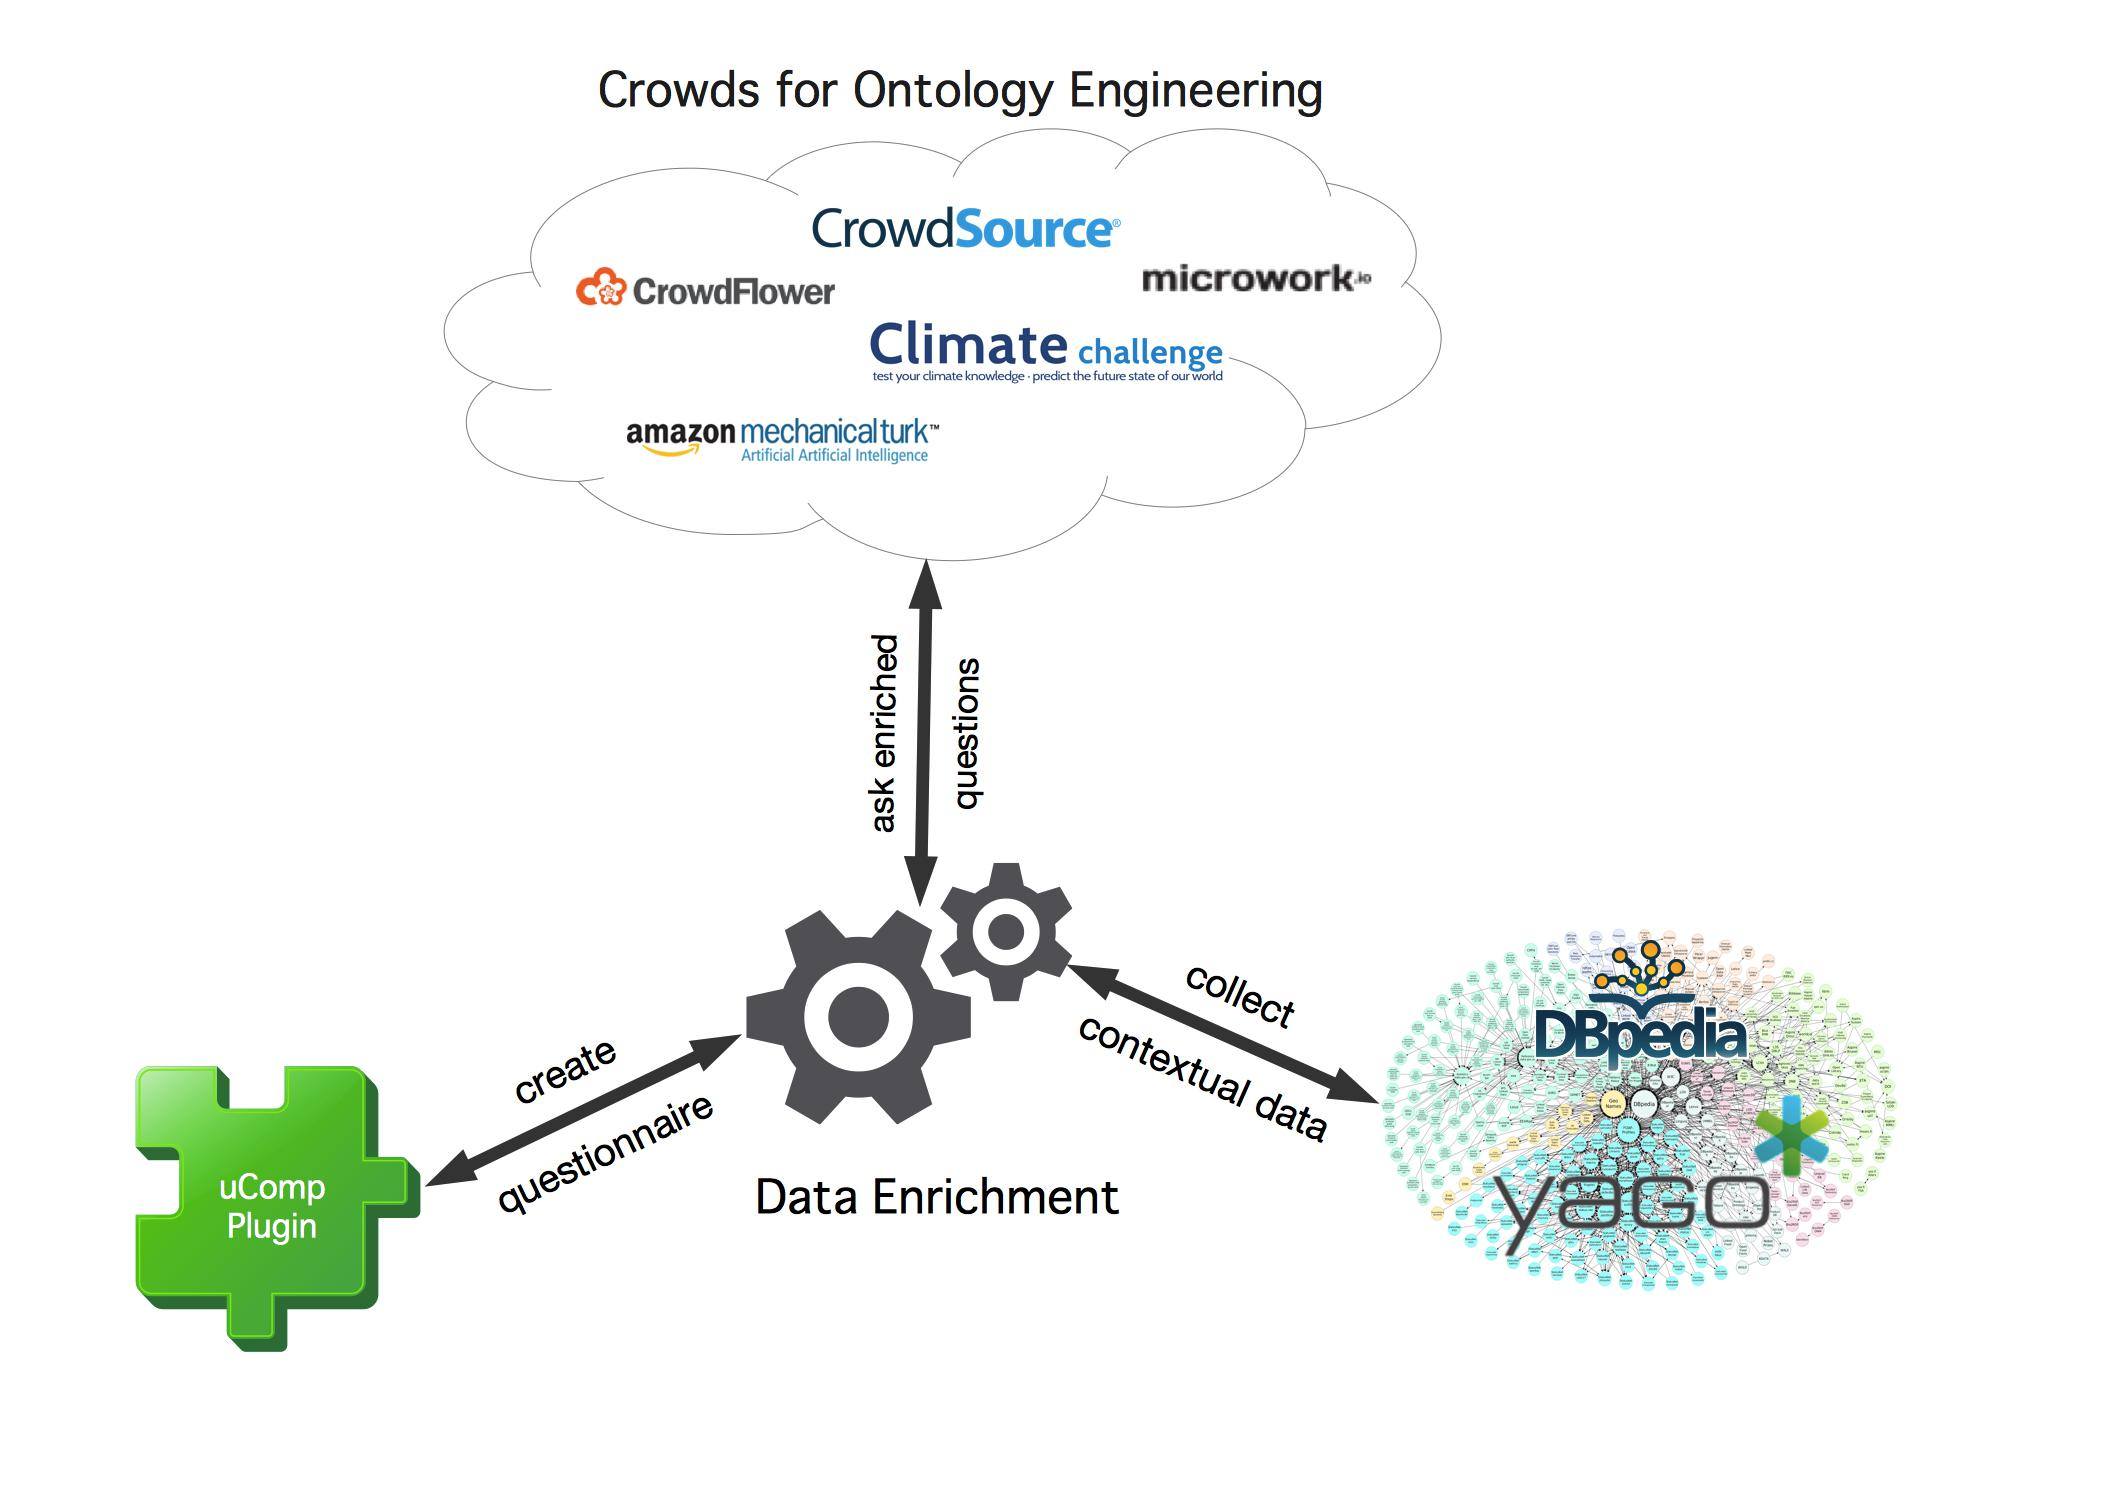
\includegraphics[width=\textwidth]{graphics/new_architecture}
	 \caption{Basic workflow in adding contextual data to crowdsourcing tasks}\label{fig:new_architecture}
\end{figure}

\section{State of the art}
\paragraph{Crowdsourcing}
In recent years an emerging research area was Crowdsourcing Systems~(CS~Systems) with the purpose of solving problems which are challenging for machines but easy for humans. Although most CS~Systems are included in this definition, there is no agreement in the research community whether platforms such as online encyclopedias~(e.g. Wikipedia\footnote{\url{https://www.wikipedia.org/}}) or collaboration boards~(e.g. StackOverflow\footnote{\url{https://stackoverflow.com/}}) should be classified as CS~Systems~\cite{crowdsourcingsystems2011}. 
This paper also highlights four major challenges inherent to \emph{any} CS~System: 
\begin{inparaenum}[1)]
		\item how to recruit and retain users, 
		\item what can users do, 
		\item how to combine their inputs and
		\item how to evaluate them
\end{inparaenum}.
Even though several CS~Systems have addressed these challenges, there is little analysis evaluating task design, marketplace dynamics and worker behavior in a broader context~\cite{jain2017understanding}. Also, it needs more research in the direction of a more complete approach, facing the challenge of motivating users and taking all aspects of a CS~System into account~\cite{truong2016incentive}. 
\paragraph{Crowdsourcing in the Semantic Web}
Due to the nature of ontology engineering tasks which are often context-specific and require domain expertise, it seems obvious that crowdsourcing is an option for solving ontology related tasks efficiently. \citet{siorpaes2008games} identified three major stages of the Semantic Web Lifecycle, each supporting different aspects of an ontology engineering workflow. These stages include 
\begin{inparaenum}[1)]
		\item \emph{Building and maintaining Semantic Web vocabularies},
		\item \emph{Aligning Semantic Web vocabularies} and
		\item \emph{Annotating content and maintaining annotations}.
\end{inparaenum}

Combining the two disciplines Crowdsourcing and Semantic Web is a relatively new research field, creating new opportunities for future research. \citet{sarasua2015crowdsourcing} summarized current research challenges and provided scenarios facilitating the interplay between these disciplines. As there exist not much literature on this topic, they encouraged the research community to establish principles and best practices to foster the integration of Crowdsourcing into Semantic Web technologies. 

\paragraph{The uComp Protege Plugin}
The initial architecture for improving ontology engineering tasks with the help of crowdsourcing that will be used as a baseline for this thesis was introduced by \citet{wohlgenannt2016crowd}. The authors reported that \enquote{its use reduces the working times for the ontology engineers 11 times, lowers the overall task costs by 40\% to 83\% depending on the crowdsourcing settings used and leads to data quality comparable with that of tasks performed by ontology engineers.} The overall workflow ranging from task specification to result interpretation and presentation used by the tool is shown in Figure~\ref{fig:ucomp_workflow}.
% Describe the need for context [Mortensen]

\paragraph{Enrichment of crowdsourcing tasks with contextual data}
We limit our research to two related approaches described below. Even though these were applied in different research contexts, applicability can be broadened to include descriptions in crowdsourcing tasks.

One area of interest is ontology matching. \citet{hoffmann2010context} states that \enquote{the context of an ontology can be given by its relations with other ontologies}. Hence, ontology matching is the task of putting ontologies in context whereas content based matching uses its metadata~(e.g. comments, labels, properties, \ldots) to compare ontologies. The context-based matcher Scarlet, first introduced by~\citet{sabou2008scarlet} and extended by~\citet{hoffmann2010context} combines various parameters of context-based matching such as the kind of ontologies that will be used, the method to choose ontologies to anchor concepts, the method to contextualize, the method to aggregate distinct results. 

Another area of interest is Question~Answering~Systems~(QA-Systems). Instead of using a formal query language like SPARQL~\cite{harris2013sparql}, QA-Systems process queries written in natural language. A rather complete overview of QA-Systems in the context of the Semantic Web covering major challenges is given by~\citet{hoffner2016survey}. They identified several challenges such as \emph{Lexical Gap}, \emph{Ambiguity}, \emph{Multilingualism}, \emph{Complex Queries}, \emph{Distributed Knowledge} and \emph{Procedural-,~Temporal-~and~Spatial~Questions}. They concluded that these challenges were subject of active research, leaving room for future improvements. 

\begin{figure}[H]
	 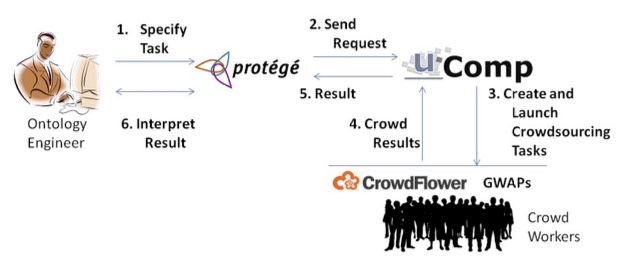
\includegraphics[width=\textwidth]{graphics/ucomp_workflow}
	 \caption{Overall workflow of the uComp Protege Plugin~\cite{wohlgenannt2016crowd}}\label{fig:ucomp_workflow}
\end{figure}

\section{Relation to Software Engineering \& Internet Computing}
Researching, evaluating, developing, analyzing and verifying are important skills in the study \emph{Software Engineering \& Internet Computing}, matching the required skillset for answering the research questions in this thesis. Moreover, the development of an extension of the uComp Protege plugin requires an in-depth understanding of all phases of the Software Development Lifecycle, including Requirement~Analysis, Design, Implementation and Maintenance. Furthermore, an overall understanding of scientific principles and approaches as well as advanced knowledge of ontologies and related concepts is necessary. Therefore the qualification profile in the study of \emph{Software Engineering \& Internet Computing} is well covered. 

The following courses in the study of \emph{Software Engineering \& Internet Computing} are relevant:
\begin{itemize}
	\item 183.243 Advanced Software Engineering (PR)
	\item 180.456 Advanced Software Engineering (VO)
	\item 188.399 Introduction to Semantic Web
	\item 188.409 Requirements Engineering and Specification
\end{itemize}

\newpage
\bibliography{literature}
\bibliographystyle{plainnat}

\end{document}